\chapter{Virtual Private Networks (VPN) and IPsec}

\section{VPN introduction}

A VPN is a private network that is created over a public network, usually the Internet. A VPN is virtual because it carries information within a private network, but that information is actually transported over a public network. A VPN is private in that the traffic is encrypted to keep the data confidential while it is transported across the public network.\\

In the simplest sense, a VPN connects two endpoints, such as two remote offices, over a public network to form a logical connection. The logical connections can be made at either Layer 2 or Layer 3. This chapter focuses on Layer 3 VPN technology. Common examples of Layer 3 VPNs are GRE, Multiprotocol Label Switching (MPLS), and IPsec (This course focuses on IPsec VPNs).\\

\begin{figure}[hbtp]
\caption{Remote-access VPN}\label{RemoteVPN}
\centering
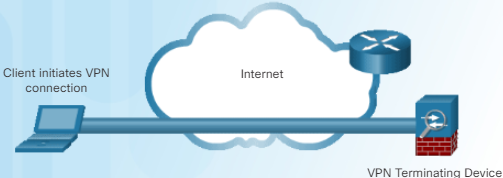
\includegraphics[scale=0.5]{pictures/RemoteVPN.PNG}
\end{figure}

\begin{figure}[hbtp]
\caption{Site-to-site VPN}\label{Site2site}
\centering
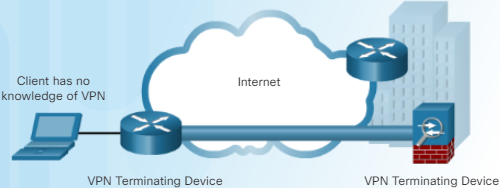
\includegraphics[scale=0.5]{pictures/Site2site.PNG}
\end{figure}


There are two basic types of VPNs: remote-access and site-to-site. A \textbf{remote-access VPN} is created when VPN connection is dynamically created and can be enabled and disabled when needed (Figure \ref{RemoteVPN}). A \textbf{site-to-site VPN} is static and devices on both sides of the VPN connection are aware of the VPN configuration in advance. However, internal hosts have no knowledge that a VPN exists (Figure \ref{Site2site}).\\

\begin{figure}[hbtp]
\caption{Hairspinning}\label{Hairspinning}
\centering
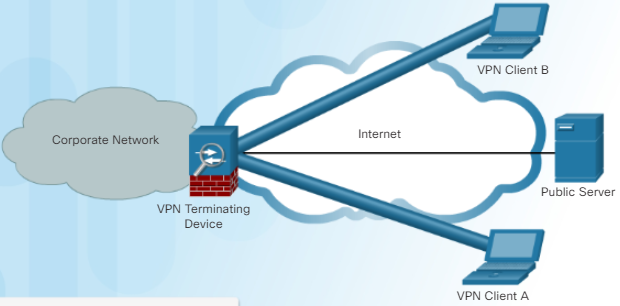
\includegraphics[scale=0.5]{pictures/Hairspinning.PNG}
\end{figure}

\begin{figure}[hbtp]
\caption{Split Tunneling}
\centering
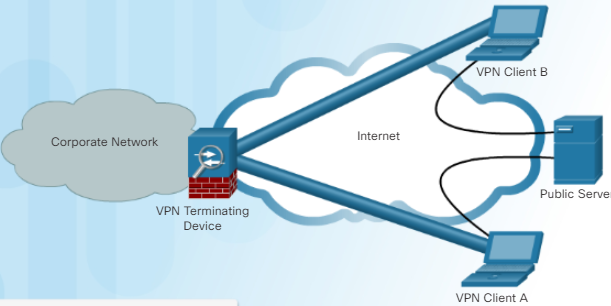
\includegraphics[scale=0.5]{pictures/SplitTunneling.PNG}
\end{figure}



\textbf{Hairpinning} is a situation in which the VPN terminating device at the corporate network is the hub and the remote-access VPN clients are spokes (Figure \ref{Hairspinning}). In \textbf{Split tunneling}, if traffic is destined for a corporate subnet, it is sent through the VPN tunnel; otherwise, it is sent as unencrypted traffic (untrusted) to the Internet.

\section{IPsec introduction}

IPsec is an IETF standard that defines how a VPN can be secured across IP networks. IPsec is not bound to any specific rules for secure communications (Figure \ref{IPsecFramework}). This flexibility of the framework allows IPsec to easily integrate new security technologies without updating the existing IPsec standards. The level of security and reliability is increased from left to right, meaning that the right-most is the most secure and reliable.\\

\begin{figure}[hbtp]
\caption{IPsec framework}\label{IPsecFramework}
\centering
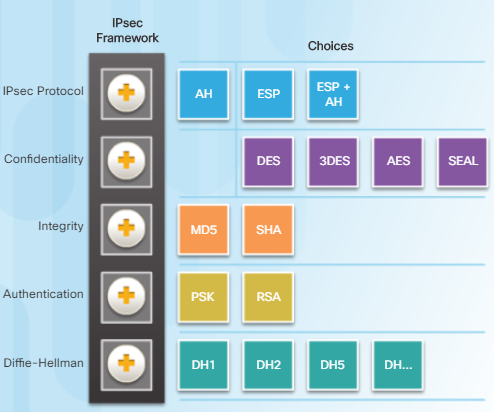
\includegraphics[scale=0.5]{pictures/IPsecFramework.PNG}
\end{figure}

\begin{figure}[hbtp]
\caption{IPsec implementations}\label{SAexample}
\centering
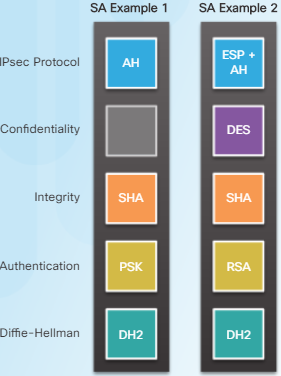
\includegraphics[scale=1]{pictures/SAexample.PNG}
\end{figure}


Figure \ref{SAexample} shows examples of security associations (SAs) for two different implementations. An SA is the basic building block of IPsec. When establishing a VPN link, the peers must share the same SA. 

\section{IPsec protocols}

Having said that IPsec framework contains a variety of protocols. This section introduce Authentication Header (AH) protocol and Encapsulation Security Protocol (ESP). Refer to figure \ref{IPsecFramework}, you can see that AH and ESP are both IPsec protocols, the first layer of IPsec framework.

\subsection{Authentication Header (AH) protocol}

AH achieves \textbf{authenticity} by applying a \textbf{keyed one-way} hash function to the packet to create a hash or message digest. AH supports MD5 and SHA algorithms. AH may not work if the environment uses NAT. The AH process occurs in this order:

\begin{figure}[hbtp]
\caption{Authentication header (AH) process}\label{AHproto}
\centering
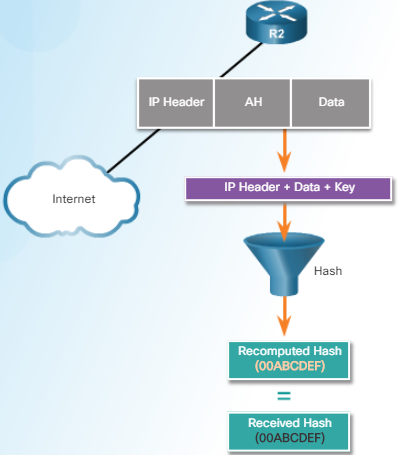
\includegraphics[scale=1]{pictures/AHproto.PNG}
\end{figure}


\begin{enumerate}
\item The IP header and data payload are hashed using the shared secret key.

\item The hash builds a new AH header, which is inserted into the original packet (Figure 2).

\item The new packet is transmitted to the IPsec peer router.

\item The peer router hashes the IP header and data payload using the shared secret key, extracts the transmitted hash from the AH header, and compares the two hashes (Figure \ref{AHproto}). The hashes must match exactly. 
\end{enumerate}

\subsection{Encapsulation Security Protocol (ESP)}

ESP provides \textbf{confidentiality} by encrypting the entire original IP datagram and ESP trailer. If ESP is selected as the IPsec protocol, an encryption algorithm must also be selected. The default algorithm for IPsec is 56-bit DES. ESP can also provide \textbf{integrity} and \textbf{authentication}.\\

\begin{figure}[hbtp]
\caption{Encryption and Authentication with ESP}\label{ESP}
\centering
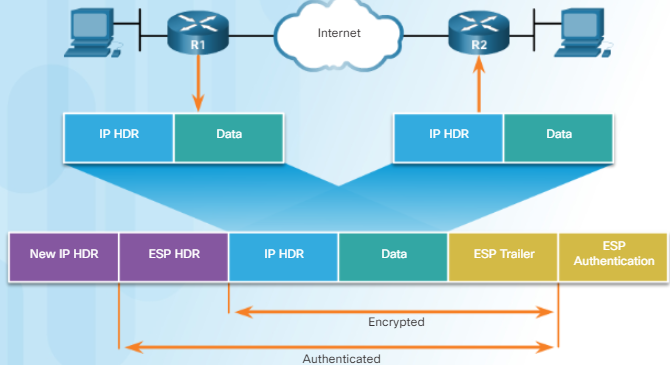
\includegraphics[scale=1]{pictures/ESP.PNG}
\end{figure}


Optionally, ESP can also enforce anti-replay protection. \textbf{Anti-replay protection} verifies that each packet is unique and is not duplicated. This protection ensures that a hacker cannot intercept packets and insert changed packets into the data stream. Anti-replay works by keeping track of packet sequence numbers and using a sliding window on the destination end.\\

Looking at figure \ref{ESP}, ESP process starts with encrypting the payload (IP datagram and ESP trailer). Then, the newly encrypted data and the ESP header are included in the hashing process. Next, a new IP header is attached to the authenticated payload. The new IP address is used to route the packet through the Internet.\\

\subsection{Transport and Tunnel modes}

ESP and AH can be applied to IP packets in two different modes, transport mode and tunnel mode. \\

In \textbf{ESP transport mode}, security is provided only for the transport layer of the OSI model and above. Transport mode protects the payload of the packet but leaves the original IP address in plaintext. The original IP address is used to route the packet through the Internet. ESP transport mode is used between hosts.\\

\textbf{ESP tunnel mode} provides security for the complete original IP packet. The original IP packet is encrypted and then it is encapsulated in another IP packet. This is known as IP-in-IP encryption. The IP address on the outside IP packet is used to route the packet through the Internet. ESP tunnel mode is used between a host and a security gateway, or between two security gateways.\\

\textbf{AH transport mode} provides authentication and integrity for the entire packet. It does not encrypt the data, but it is protected from modification.\\

\textbf{AH tunnel mode} encapsulates the IP packet with an AH and a new IP header, and signs the entire packet for integrity and authentication.

\section{IPsec key exchange}

\subsection{IKE protocol}

The Internet Key Exchange (IKE) protocol is a key management protocol standard. IKE is used in conjunction with the IPsec standard. IKE automatically negotiates IPsec security associations and enables IPsec secure communications. \\

Instead of transmitting keys directly across a network, IKE calculates shared keys based on the exchange of a series of data packets. This disables a third party from decrypting the keys even if the third party captured all of the exchanged data that was used to calculate the keys.\\

IKE uses \textbf{UDP port 500} to exchange IKE information between the security gateways. UDP port 500 packets must be permitted on any IP interface that is connecting a security gateway peer.

%\subsection{IKE phase 1: Negotiate \emph{ISAKMP} SA policy}

%\begin{figure}[hbtp]
%\caption{IKE phase 1 -- Negotiate ISAKMP policy}\label{IKEphase1}
%\centering
%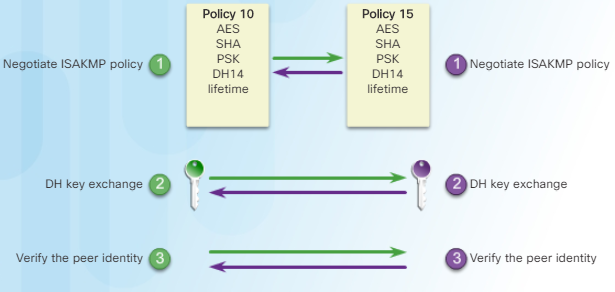
\includegraphics[scale=1]{pictures/IKEphase1.PNG}
%\end{figure}
%
%In Phase 1 (figure \ref{IKEphase1}), the following tasks are performed in order:
%
%\begin{enumerate}
%\item IPsec peers authenticate each other. 
%\item Negotiate a ISAKMP SA policy
%\item Set up a secure tunnel between the peers. This tunnel will then be used in Phase 2.
%\end{enumerate}

%two IPsec peers perform the initial negotiation to ensure that SAs (ISAKMP policy) on both sides are matched. This phase also authenticates the peers, and sets up a secure tunnel between the peers. \\

%Phase 1 can be implemented in main mode or aggressive mode. When \textbf{main mode} is used, the identities of the two IKE peers are hidden. \textbf{Aggressive mode} takes less time than main mode to negotiate keys between peers. However, since the authentication hash is sent unencrypted before the tunnel is established, aggressive mode is vulnerable to brute-force attacks.

%\subsection{IKE phase 2: Negotiate the \emph{IPsec} SA policy}

%The purpose of IKE Phase 2 is to negotiate the IPsec SA policy (figure \ref{IKEphase2}). IKE Phase 2 can only occur after IKE has established a secure tunnel in Phase 1.  

%\begin{figure}[hbtp]
%\caption{IKE phase 2 -- Negotiate IPsec policy for sending secure traffic accross the tunnel}\label{IKEphase2}
%\centering
%
\includegraphics[scale=1]{pictures/IKEphase2.PNG}
%\end{figure}

%Quick mode also renegotiates a new IPsec SA when the IPsec SA lifetime expires. Basically, quick mode refreshes the keying material that creates the shared secret key. This is based on the keying material that is derived from the DH exchange in Phase 1.

\subsection{IPsec negotiation}
IPsec negotiation to establish a VPN involves five steps, which include IKE Phase 1 and Phase 2:

\begin{enumerate}
\item \textbf{ISAKMP tunnel:}  When host A sends ``interesting'' traffic to host B, an ISAKMP tunnel is initiated. Traffic is considered interesting when it travels between the peers and meets the criteria that are defined in an ACL.

\item \textbf{IKE Phase 1:} The peers negotiate the ISAKMP SA policy. When the peers agree on the policy and are authenticated, a secure tunnel is created.

\item \textbf{IKE Phase 2:} The IPsec peers use the tunnel created in IKE phase 1 to negotiate the IPsec SA policy. The negotiation of the shared policy determines how the IPsec tunnel is established. In this phase, a separate key exchange is required for each data flow.

\item The IPsec tunnel is created, and data is transferred between the IPsec peers based on the IPsec SAs.

\item The IPsec tunnel terminates when the IPsec SAs are manually deleted, or when their lifetime expires.
\end{enumerate}

\section{Site-to-site IPsec configuration}

\begin{figure}[hbtp]
\caption{Site-to-site VPN topology}\label{VPNtopolgy}
\centering
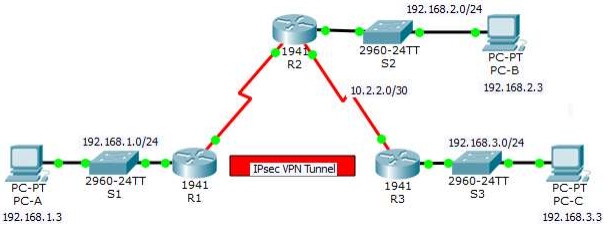
\includegraphics[scale=0.5]{pictures/VPNtopolgy.PNG}
\end{figure}

The configuration tasks for the topology in figure \ref{VPNtopolgy} are shown in order as below:

\begin{enumerate}
\item Test connectivity
\item Enable the Security Technology package
\item Identify interesting traffic: Configure ACL to identify the traffic from the LAN on R1 to the LAN on R3 as interesting. This interesting
traffic will trigger the IPsec VPN to be implemented when there is traffic between the R1 to R3 LANs.
\item Configure the IKE Phase 1 policy on R1. Use the mnemonic \textbf{HAGLE} to remember the five SAs to configure: Hash, Authentication, Group, Lifetime, and Encryption. Note that the address of the peer router R3 is the address of serial interface connected to the Internet (s0/0/0).
\item Configure the IKE Phase 2 IPsec policy on R1. First, we create the transform-set VPN-SET to use esp-aes and esp-sha-hmac. Next, a crypto map VPN-MAP is created to bind all of the Phase 2 parameters together. Use sequence number 10 and identify it as an ipsec-isakmp map. In the following commands,the perfect forwarding secrecy type is set using the \code{set pfs} command.
\item Configure the crypto map on the outgoing interface.
\item Repeat the above steps on R3.
\end{enumerate}

\begin{sexylisting}{Site-to-site IPsec}
#STEP 2
license boot module c1900 technology-package securityk9

#STEP 3
access-list 110 permit ip 192.168.1.0 0.0.0.255 192.168.3.0 0.0.0.255

#STEP 4
crypto isakmp policy 10
	hash sha 
	authentication pre-share
	group 14
	lifetime 3600
	encryption aes 256
	exit
crypto isakmp key vpnpa55 address 10.2.2.2	

#STEP 5
crypto ipsec transform-set VPN-SET esp-aes esp-sha-hmac
crypto map VPN-MAP 10 ipsec-isakmp
	description VPN connection to R3
	set peer 10.2.2.2
	set transform-set VPN-SET
	set pfs group14
	set security-association lifetime seconds 900 
	match address 110
	exit

#STEP 6
interface s0/0/0
	crypto map VPN-MAP
	exit

#VERIFICATION
show crypto ipsec transform-set 
show crypto map
show crypto isakmp sa
show crypto ipsec sa		
\end{sexylisting}
